% -*- coding: utf-8 -*-
% !TEX program = xelatex

\documentclass[9pt]{beamer}

\usetheme[style=beta]{epyt} % alpha, beta, delta, gamma, zeta
% \usetheme{Warsaw}
\usepackage[UTF8,noindent]{ctex}
% ######### DEFINE COLOR ###############
\definecolor{blue}{rgb}{0.0,0.0,1.0}
\definecolor{red}{rgb}{1.0,0.0,0.0}
\definecolor{purple}{rgb}{0.75, 0.0, 1.0}

\def\blue{\textcolor{blue}}
\def\red{\textcolor{red}}
\def\purple{\textcolor{purple}}


\def\ds{\displaystyle}
\def\cd{\cdots}
\def\dd{\ddots}
\def\vd{\vdots}
\def\id{\iddots}
\def\ft{\frametitle}
\def\diag{\mathrm{diag}}
\def\Im{\mathrm{Im~}}
\def\Ker{\mathrm{Ker~}}

\def\MA{\boldsymbol{A}}
\def\MB{\boldsymbol{B}}
\def\MC{\boldsymbol{C}}
\def\MD{\boldsymbol{D}}
\def\ME{\boldsymbol{E}}
\def\MF{\boldsymbol{F}}
\def\MH{\boldsymbol{H}}
\def\MI{\boldsymbol{I}}
\def\MP{\boldsymbol{P}}
\def\MQ{\boldsymbol{Q}}
\def\MR{\boldsymbol{R}}
\def\MS{\boldsymbol{S}}
\def\MT{\boldsymbol{T}}
\def\MU{\boldsymbol{U}}
\def\MX{\boldsymbol{X}}
\def\MY{\boldsymbol{Y}}
\def\MZ{\boldsymbol{Z}}
\def\M0{\boldsymbol{0}}
\def\MLambda{\boldsymbol{\Lambda}}

\def\R{\mathbb R}
\def\C{\mathbb C}
\def\dim{\mathrm{dim~}}
\def\rank{\mathrm{r}}
\def\tr{\mathrm{tr}}
\def\det{\mathrm{det}}
\def\vn{{\boldsymbol{n}}}
\def\vx{{\boldsymbol{x}}}
\def\vy{{\boldsymbol{y}}}
\def\vz{{\boldsymbol{z}}}
\def\va{{\boldsymbol{a}}}
\def\vb{{\boldsymbol{b}}}
\def\ve{{\boldsymbol{e}}}
\def\vi{{\boldsymbol{i}}}
\def\vj{{\boldsymbol{j}}}
\def\vk{{\boldsymbol{k}}}
\def\vu{{\boldsymbol{u}}}
\def\vv{{\boldsymbol{v}}}

\def\tf{\ttfamily}
\def\Lambdabd{\boldsymbol{\Lambda}}
\def\alphabd{\boldsymbol{\alpha}}
\def\betabd{\boldsymbol{\beta}}
\def\gammabd{\boldsymbol{\gamma}}
\def\xibd{\boldsymbol{\xi}}
\def\zetabd{\boldsymbol{\zeta}}
\def\etabd{\boldsymbol{\eta}}
\def\epsilonbd{\boldsymbol{\epsilon}}
\def\phibd{\boldsymbol{\phi}}
\def\varphibd{\boldsymbol{\varphi}}
\def\sigmabd{\boldsymbol{\sigma}}
\def\omegabd{\boldsymbol{\omega}}
\def\taubd{\boldsymbol{\tau}}
%\def\rank{\boldsymbol{rank}}
\usepackage{amsmath,amsthm,amssymb,mathdots}
\usepackage{fourier}
\usepackage{multicol}
%\usepackage{fontspec}
\usepackage{subfigure}
\usepackage[most]{tcolorbox}
\newcounter{testexample}
\usepackage{xparse}
\usepackage{lipsum}
\usepackage[UTF8,noindent]{ctex}
\usepackage{extarrows}
%\usepackage{courier}
\usepackage{animate}
\usepackage{dcolumn}
\usepackage{pgf}
\usepackage{tikz}
\usetikzlibrary{calc}
\usetikzlibrary{arrows,snakes,backgrounds,shapes,patterns}
\usetikzlibrary{matrix,fit,positioning,decorations.pathmorphing}
\usepackage{listings}
\lstset{
        language=c,
        keywordstyle=\color{red},
        frame=tb,
        basicstyle=\ttfamily,
        commentstyle=\small\color{blue},
        breakindent=0pt,
        rulesepcolor=\color{red!20!green!20!blue!20},
        rulecolor=\color{black},
        tabsize=4,
        numbersep=5pt,
        breaklines=true,
        backgroundcolor=\color{red!10},
        showstringspaces=false,
        showspaces=false,
        showtabs=false,
        extendedchars=false,
        escapeinside=``,
}

\usepackage{refcount}
\usepackage{multicol}
\newcounter{countitems}
\newcounter{nextitemizecount}
\newcommand{\setupcountitems}{%
	\stepcounter{nextitemizecount}%
	\setcounter{countitems}{0}%
	\preto\item{\stepcounter{countitems}}%
}
\makeatletter
\newcommand{\computecountitems}{%
	\edef\@currentlabel{\number\c@countitems}%
	\label{countitems@\number\numexpr\value{nextitemizecount}-1\relax}%
}
\newcommand{\nextitemizecount}{%
	\getrefnumber{countitems@\number\c@nextitemizecount}%
}
\newcommand{\previtemizecount}{%
	\getrefnumber{countitems@\number\numexpr\value{nextitemizecount}-1\relax}%
}
\makeatother    
\newenvironment{AutoMultiColItemize}{%
	\ifnumcomp{\nextitemizecount}{>}{3}{\begin{multicols}{2}}{}%
		\setupcountitems\begin{itemize}}%
		{\end{itemize}%
		\unskip\computecountitems\ifnumcomp{\previtemizecount}{>}{3}{\end{multicols}}{}}

\input{../asset/global_newenviroment}
\renewcommand{\proofname}{\textbf{证明}}
\newtheorem{li}{例}%[section]
%\newtheorem*{li*}{例}
\newtheorem{lianxi}{练习}
\newtheorem*{jielun}{结论}
\newtheorem*{dingli}{定理}
\newtheorem*{mingti}{{命题}} 
\newtheorem*{yinli}{{引理}} 
\newtheorem*{tuilun}{{推论}}
\newtheorem*{dingyi}{{定义}}
\newtheorem*{biancheng}{{编程}}
\newtheorem*{jie}{{解}}
\newtheorem{zhu}{{注}}
\newtheorem*{xingzhi}{{性质}}%[subsection]
\newtheorem*{wenti}{{问题}}
\newtheorem*{rem}{{Remark}}
\newtheorem*{lem}{{Lemma}}



\begin{document}

\title{向量空间与线性变换}
%\subtitle{行列式}
\author{张晓平}
\institute{武汉大学数学与统计学院}


\begin{frame}[plain]\transboxout
  \titlepage
\end{frame}

\section*{目录}
\frame{  
  \frametitle{\secname}
%  \begin{multicols}{2}  %两行目录
    \tableofcontents
%  \end{multicols}
}
\AtBeginSection[] {  %在每个subsection前面显示一次目录
  \frame{
%    \begin{multicols}{2}  %两行目录
      \tableofcontents[current,currentsection]
%    \end{multicols}
  }
}

\AtBeginSubsection[] {  %在每个subsection前面显示一次目录
  \frame{
%    \begin{multicols}{2}  %两行目录
      \tableofcontents[current,currentsubsection]
%    \end{multicols}
  }
}
 
\section{二次型的定义与矩阵表示\quad 合同矩阵}

\begin{frame}
  
    \begin{dingyi}[二次型]
      $n$元变量$x_1,x_2,\cd,x_n$的二次齐次多项式
      $$
      \begin{array}{rcccccccc}
        f(x_1,x_2,\cd,x_n) &=& \\[0.1in]
        a_{11}x_1^2&+&2a_{12}x_1x_2&+&2a_{13}x_1x_3&+&\cd&+&2a_{1n}x_1x_n\\[0.1in]
        &+&a_{22}x_2^2&+&2a_{23}x_2x_3&+&\cd&+&2a_{2n}x_2x_n\\[0.1in]
        &&&&\cd&&\cd\\[0.1in]
        &&&&&&&+&a_{nn}x_n^2
      \end{array}
      $$
     当系数属于数域$F$时,称为数域$F$上的一个\blue{\underline{$n$元二次型}}。
    \end{dingyi}
  
\end{frame}


\begin{frame}
  
    $$
    \begin{array}{l}
      f(x_1,x_2,\cd,x_n) =  \\[0.1in]
      \begin{array}{rcccccccccc}
        &a_{11}x_1^2&+&a_{12}x_1x_2&+&a_{13}x_1x_3&+&\cd&+&a_{1n}x_1x_n\\[0.1in]
        +&a_{21}x_2x_1&+&a_{22}x_2^2&+&a_{23}x_2x_3&+&\cd&+&a_{2n}x_2x_n\\[0.1in]
        &\cd&&\cd&&\cd&&\cd\\[0.1in]
        +&a_{n1}x_nx_1&+&a_{n2}x_nx_2&+&a_{n3}x_2x_3&+&\cd&+&a_{nn}x_n^2
      \end{array} \\[0.5in] \pause
      \ds = \sum_{i=1}^nx_i(a_{i1}x_1+a_{i2}x_2+\cd+a_{in}x_n)
      \ds = \sum_{i=1}^nx_i\sum_{j=1}^n a_{ij}x_{ij}
      \ds = \sum_{i=1}^n\sum_{j=1}^na_{ij}x_ix_j\\[0.2in] \pause
      \ds = (x_1,x_2,\cd,x_n)\left(
      \begin{array}{c}
        a_{11}x_1+a_{12}x_2+\cd+a_{1n}x_n\\
        a_{21}x_1+a_{22}x_2+\cd+a_{2n}x_n\\
        \vd\\
        a_{n1}x_1+a_{n2}x_2+\cd+a_{nn}x_n
      \end{array}
      \right)\\[0.3in]\pause
      \ds = (x_1,x_2,\cd,x_n)\left(
      \begin{array}{cccc}
        a_{11}&a_{12}&\cd&a_{1n}\\
        a_{21}&a_{22}&\cd&a_{2n}\\
        \vd&\vd&&\vd\\
        a_{n1}&a_{n2}&\cd&a_{nn}\\
      \end{array}
      \right)\left(
      \begin{array}{c}
        x_1\\
        x_2\\
        \vd\\
        x_n
      \end{array}\right) \pause = \vx^T\MA\vx
    \end{array}
    $$
  
\end{frame}


\begin{frame}
  
    \begin{itemize}
    \item
      对于任意一个二次型,总可以写成对称形式
      $$
      f(x_1,x_2,\cd,x_n)=\vx^T\MA\vx
      $$
      其中$\MA$为对称矩阵。\\[0.1in]\pause
    \item
      若$\MA,\MB$为对称矩阵,且
      $$
      f(x_1,x_2,\cd,x_n)=\vx^T\MA\vx=\vx^T\MB\vx
      $$
      则必有$\MA=\MB$。\\[0.1in]\pause
    \item 二次型和它的矩阵式相互唯一确定的,因此研究二次型的性质就转化为研究$\MA$所具有的性质。
    \end{itemize}

  
\end{frame}

\begin{frame}
  
    \begin{li}
      设$f(x_1,x_2,x_3,x_4)=2x_1^2+x_1x_2+2x_1x_3+4x_2x_4+x_3^2+5x_4^2$,则它的矩阵为
      $$
      \MA=\left(
      \begin{array}{cccc}
        2&\ds\frac12&1&0\\[0.2cm]
        \ds\frac12&0&0&2\\[0.2cm]
        1&0&1&0\\[0.2cm]
        0&2&0&5
      \end{array}
      \right)
      $$
    \end{li}
  
\end{frame}

\begin{frame}
  
    一个二次型$\vx^T\MA\vx$可看成是$n$维向量$\alphabd$的一个函数,即
    $$
    f(\alphabd)=\vx^T\MA\vx
    $$
    其中$\vx=(x_1,x_2,\cd,x_n)^T$是$\alphabd$在$\mathbb R^n$的一组基下的坐标向量,故二次型$\vx^T\MA\vx$是向量$\alphabd$的$n$个坐标的二次齐次函数。
    因此二次型作为$\alphabd$的函数,其矩阵是与一组基相联系的。
  
\end{frame}

\begin{frame}
  
    设$\alphabd$在两组基$\{\epsilonbd_1,\epsilonbd_2,\cd,\epsilonbd_n\}$和$\{\etabd_1,\etabd_2,\cd,\etabd_n\}$下的坐标向量分别为
    $$
    \vx=(x_1,x_2,\cd,x_n)^T\mbox{~~和~~}\vy=(y_1,y_2,\cd,y_n)^T
    $$
    又
    $$
    (\etabd_1,\etabd_2,\cd,\etabd_n)=(\epsilonbd_1,\epsilonbd_2,\cd,\epsilonbd_n)\MC
    $$
    故
    $$
    \vx=\MC\vy
    $$
    从而
    $$
    f(\alphabd)=\vx^T\MA\vx=\vy^T(\MC^T\MA\MC)\vy
    $$ \pause


    \blue{
      二次型$f(\alphabd)$在两组基$\{\epsilonbd_1,\epsilonbd_2,\cd,\epsilonbd_n\}$和$\{\etabd_1,\etabd_2,\cd,\etabd_n\}$下所对应的矩阵分别为
      $$
      \MA \mbox{~~和~~} \MC^T\MA\MC     
      $$
    }
  
\end{frame}


\begin{frame}
  
    \begin{li}
      设$\alphabd$在自然基$\{\epsilonbd_1,\epsilonbd_2\}$下的坐标$(x_1,x_2)^T$满足方程
      \begin{equation}\label{li2-1}
        5x_1^2+5x_2^2-6x_1x_2=4.
      \end{equation}      
      将$\epsilonbd_1,\epsilonbd_2$逆时针旋转$\pi/4$变为$\etabd_1,\etabd_2$      
    \end{li}
    \pause 
    $$
    (\etabd_1,\etabd_2)=(\epsilonbd_1,\epsilonbd_2)\left(
    \begin{array}{rr}
      \cos \pi/4&-\sin \pi/4\\
      \sin\pi/4&\cos\pi/4
    \end{array}
    \right)
    $$
    则$\alphabd$在基$\{\etabd_1,\etabd_2\}$下的坐标$(y_1,y_2)^T$满足
    $$
    \vx=\left(
    \begin{array}{c}
      x_1\\
      x_2
    \end{array}
    \right)=\left(
    \begin{array}{rr}
      \cos \pi/4&-\sin \pi/4\\
      \sin\pi/4&\cos\pi/4
    \end{array}
    \right)\left(
    \begin{array}{c}
      y_1\\
      y_2
    \end{array}
    \right)=\MC\vy
    $$\pause 
    (\ref{li2-1})的矩阵形式为
    $$
    \vx^T\MA\vx=(x_1,x_2)\left(
    \begin{array}{rr}
      5&-3\\
      -3&5
    \end{array}
    \right)\left(
    \begin{array}{c}
      x_1\\
      x_2
    \end{array}
    \right)=4
    $$

  
\end{frame}


\begin{frame}
  
    $$
    \begin{array}{rl}
      \vx^T\MA\vx& =\vy^T\MC^T\MA\MC\vy\\[0.1in]
      & =(y_1,y_2)\left(
      \begin{array}{rr}
        \frac{\sqrt{2}}2&\frac{\sqrt{2}}2\\[0.2cm]
        -\frac{\sqrt{2}}2&\frac{\sqrt{2}}2
      \end{array}
      \right)\left(
      \begin{array}{rr}
        5&-3\\
        -3&5
      \end{array}
      \right)\left(
      \begin{array}{rr}
        \frac{\sqrt{2}}2&-\frac{\sqrt{2}}2\\[0.2cm]
        \frac{\sqrt{2}}2&\frac{\sqrt{2}}2
      \end{array}
      \right)\left(
      \begin{array}{c}
        y_1\\
        y_2
      \end{array}
      \right)\\[0.2in]
      & =(y_1,y_2)\left(
      \begin{array}{rr}
        2&0\\
        0&8
      \end{array}
      \right)\left(
      \begin{array}{c}
        y_1\\
        y_2
      \end{array}
      \right)  \\[0.2in]
      &= 2y_1^2+8y_2^2=4.      
    \end{array}
    $$ \pause
    此时,方程(\ref{li2-1})化成了在基$\{\etabd_1,\etabd_2\}$的坐标系下的标准方程,其图形是一个椭圆。

  
\end{frame}


\begin{frame}
  
    把一般的二次型$f(x_1,x_2,\cd,x_n)$化为$y_1,y_2,\cd,y_n$的纯平方项之代数和的基本方法是做坐标变换
    $$
    \vx=\MC\vy \mbox{~~~~~($\MC$为可逆矩阵)}
    $$
    使得
    $$
    \vx^T\MA\vx=\vy^T\MC^T\MA\MC\vy=d_1y_1^2+\cd+d_ny_n^2.
    $$
    \pause \vspace{0.1in}

    从矩阵的角度来说,就是对于一个实对称矩阵$\MA$,寻找一个可逆矩阵,使得$\MC^T\MA\MC$称为对角形。
  
\end{frame}


\begin{frame}
  
    \begin{dingyi}[矩阵的合同]
      对于两个矩阵$\MA$和$\MB$,若存在可逆矩阵$\MC$,使得
      $$
      \MC^T\MA\MC=\MB,
      $$
      就称$\MA$合同于$\MB$,记作$\MA\simeq\MB$。
    \end{dingyi}
  
\end{frame}



\section{化二次型为标准型}

\begin{frame}
  
    \begin{itemize}
    \item 含平方项而不含混合项的二次型称为标准二次型。\\[0.2cm]
    \item 化二次型为标准型,就是对实对称矩阵$\MA$,寻找可逆阵$\MC$,使$\MC^T\MA\MC$成为对角矩阵。
    \end{itemize}
  
\end{frame}


\subsection{$\MR^n$中向量的内积,欧式空间}

\begin{frame}  
  \begin{dingyi}
    在$\MR^n$中,对于$\alphabd=(a_1,a_2,\cd,a_n)^T$和$\betabd=(b_1,b_2,\cd,b_n)^T$,规定$\alphabd$和$\betabd$的内积为
    $$
    (\alphabd,\betabd)=a_1b_1+a_2b_2+\cd+a_nb_n.
    $$
  \end{dingyi}
  当$\alphabd$和$\betabd$为列向量时,
  $$
  (\alphabd,\betabd)=\alphabd^T\betabd=\betabd^T\alphabd.
  $$
  
\end{frame}

\begin{frame}
  
  \begin{xingzhi}[内积的运算性质]
    对于$\alphabd,\betabd,\gammabd\in\MR^n$和$k\in\MR$,
    \begin{itemize}
    \item[(i)]   $(\alphabd,\betabd)=(\betabd,\alphabd)$
    \item[(ii)]  $(\alphabd+\betabd,\gammabd)=(\alphabd,\gammabd)+(\betabd,\gammabd)$
    \item[(iii)] $(k\alphabd,\betabd)=k(\alphabd,\betabd)$
    \item[(iv)]  $(\alphabd,\alphabd)\ge0$, 等号成立当且仅当$\alphabd=\M0$.
    \end{itemize}
  \end{xingzhi}
  \pause
  \begin{dingyi}[向量长度]
    向量$\alphabd$的长度定义为
    $$
    \|\alphabd\|=\sqrt{(\alphabd,\alphabd)}
    $$
  \end{dingyi}
  
\end{frame}


\begin{frame}
  
  \begin{dingli}[柯西-施瓦茨(Cauchy-Schwarz)不等式]
    $$
    |(\alphabd,\betabd)|\le\|\alphabd\|\|\betabd\|
    $$
  \end{dingli}
  \pause 
  \proofname
  $\forall t \in \MR$,有
  $$
  (\alphabd+t\betabd,\alphabd+t\betabd) \ge 0
  $$
  即
  $$
  (\betabd,\betabd)t^2+2(\alphabd,\betabd)t+(\alphabd,\alphabd)\ge0
  $$
  此为关于$t$的二次函数,由一元二次方程理论可知
  $$
  \Delta = b^2-4ac = 4 (\alphabd,\betabd)^2-4(\alphabd,\alphabd)(\betabd,\betabd)\le 0
  $$
  即
  $$
  (\alphabd,\betabd)^2\le (\alphabd,\alphabd)(\betabd,\betabd)
  $$
  亦即
  $$
  |(\alphabd,\betabd)|\le\|\alphabd\|\|\betabd\|
  $$
  
\end{frame}

\begin{frame}
  
  \begin{dingyi}[向量之间的夹角]
    向量$\alphabd,\betabd$之间的夹角定义为
    $$
    <\alphabd,\betabd>=\arccos\frac{(\alphabd,\betabd)}{\|\alphabd\|\|\betabd\||}
    $$
  \end{dingyi}
  \pause
  \begin{dingli}
    $$\alphabd\perp\betabd ~~\Longleftrightarrow~~
    (\alphabd,\betabd)=0
    $$
  \end{dingli}
  \pause
  注意:零向量与任何向量的内积为零,从而零向量与任何向量正交。
  
\end{frame}



\begin{frame}
  
  \begin{dingli}[三角不等式]
    $$
    \|\alphabd+\betabd\|\le\|\alphabd\|+\|\betabd\|.
    $$
  \end{dingli}
  \pause\proofname
  $$
  \begin{array}{rl}
    (\alphabd+\betabd,\alphabd+\betabd)
    &= (\alphabd,\alphabd)+2(\alphabd,\betabd)+(\betabd,\betabd)\\[0.1in]
    &\le (\alphabd,\alphabd)+2|(\alphabd,\betabd)|+(\betabd,\betabd) \\[0.1in]
    &\le \|\alphabd\|^2+2\|\alphabd\|\|\betabd\|+\|\betabd\|^2 \\[0.1in]
  \end{array}
  $$
  
  \pause
  注意:当$\alphabd\perp\betabd$时,$\|\alphabd+\betabd\|=\|\alphabd\|+\|\betabd\|$。
  
\end{frame}


\begin{frame}
  
  \begin{dingyi}[欧几里得空间]
    定义了内积运算的$n$维实向量空间,称为$n$维欧几里得空间(简称欧氏空间),仍记为$\MR^n$。
  \end{dingyi}
  
\end{frame}

\subsection{配方法}


\begin{frame}
  
    \begin{li}
      用配方法把三元二次型
      $$
      f(x_1,x_2,x_3)=2x_1^2+3x_2^2+x_3^2+4x_1x_2-4x_1x_3-8x_2x_3
      $$
      化为标准型。
    \end{li}
    \pause
    \begin{jie}
    先按$x_1^2$和含$x_1$的混合项配成完全平方,即
    $$
    \begin{array}{rl}
      f(x_1,x_2,x_3)&=2[x_1^2+2x_1(x_2-x_3)+(x_2-x_3)^2]-2(x_2-x_3)^2+3x_2^2+x_3^2-8x_2x_3\\[0.1in]
      &=2(x_1+x_2-x_3)^2+x_2^2-x_3^2-4x_2x_3
    \end{array}
    $$\pause
    再按$x_2^2-4x_2x_3$配成完全平方,得
    $$
    f(x_1,x_2,x_3)=2(x_1+x_2-x_3)^2+(x_2-2x_3)^2-5x_3^2.
    $$
    \pause
    令
    $$
    \left\{
    \begin{array}{rcrcrcr}
      y_1&=&x_1&+&x_2&-&x_3\\
      y_2&=& &&x_2&-&2x_3\\
      y_3&=&&&&&x_3
    \end{array}
    \right. \pause ~~\Longrightarrow~~
    \left(
    \begin{array}{c}
      x_1\\
      x_2\\
      x_3
    \end{array}
    \right)=
    \left(
    \begin{array}{rrr}
      1&-1&-1\\
      0&1&2\\
      0&0&1
    \end{array}
    \right)
    \left(
    \begin{array}{c}
      y_1\\
      y_2\\
      y_3
    \end{array}
    \right)
    $$ \pause 
    则
    $$
    f(x_1,x_2,x_3)=2y_1^2+y_2^2-5y_3^2.
    $$
  \end{jie}
\end{frame}


\begin{frame}
  
    \begin{li}
      用配方法化二次型
      $$
      f(x_1,x_2,x_3)=2x_1x_2+4x_1x_3
      $$
      为标准型。
    \end{li}
    \pause
    \begin{jie}
    对$x_1x_2$利用平方差公式,令
    $$
    \left\{
    \begin{array}{l}
      x_1=y_1+y_2\\
      x_2=y_1-y_2\\
      x_3=y_3
    \end{array}
    \right.
    $$
    则
    $$
    f(x_1,x_2,x_3)=2(y_1+y_2)(y_1-y_2)+4(y_1+y_2)y_3=2y_1^2-2y_2^2+4y_1y_3+4y_2y_3
    $$
    \pause
    先对含$y_1$的项配完全平方,得
    $$
    f(x_1,x_2,x_3)=2(y_1^2+2y_1y_3+y_3^2)-2y_2^2-2y_3^2+4y_2y_3
    $$
    再对含$y_2$的项配完全平方,得
    $$
    f(x_1,x_2,x_3)=2(y_1+y_3)^2-2(y_2-y_3)^2
    $$
  \end{jie}
\end{frame}

\begin{frame}
  
    令
    $$
    \left\{
    \begin{array}{l}
      z_1=y_1+y_3\\
      z_2=y_2-y_3\\
      z_3=y_3
    \end{array}
    \right. ~~\Longleftrightarrow~~
    \left\{
    \begin{array}{l}
      y_1=z_1-z_3\\
      y_2=z_2+z_3\\
      y_3=z_3
    \end{array}
    \right.
    $$
    则
    $$
    f(x_1,x_2,x_3)=2z_1^2-2z_2^2.
    $$\pause
    坐标变换记为
    $$
    \vx=\MC_1\vy, \quad  \vy=\MC_2\vz, \quad \vx=\MC_1\MC_2\vz=\MC\vz
    $$
    其中
    $$
    \begin{array}{c}
      \MC_1=\left(
      \begin{array}{rrr}
        1&1&0\\
        1&-1&0\\
        0&0&1
      \end{array}
      \right),
      \quad\MC_2=\left(
      \begin{array}{rrr}
        1&0&-1\\
        0&1&1\\
        0&0&1
      \end{array}
      \right)
      \\[0.4in]
      \MC=\MC_1\MC_2=\left(
      \begin{array}{rrr}
        1&1&0\\
        1&-1&-2\\
        0&0&1
      \end{array}
      \right)      
    \end{array}
    $$
  
\end{frame}

\begin{frame}
  
    \begin{table}
      \caption{}
      \begin{tabular}{|c|c|}\hline
        二次型&对应矩阵\\\hline
        $2x_1x_2+4x_1x_3$ & $\MA=\left(
        \begin{array}{ccc}
          0&1&2\\
          1&0&0\\
          2&0&0
        \end{array}
        \right)$\\\hline
        $2z_1^2-2z_2^2$ & $\Lambdabd=\left(
        \begin{array}{ccc}
          2&&\\
          &-2&\\
          &&0
        \end{array}
        \right)$ \\\hline
      \end{tabular}      
    \end{table}
    易验证
    $$
    \MC^T\MA\MC=\diag(2,-2,0)    
    $$
  
\end{frame}

\begin{frame}
  
    任何$n$元二次型都可用配方法化为标准型,相应的变换矩阵为主对角元为1的上三角阵和对角块矩阵,或者是这两类矩阵的乘积。
  
\end{frame}


\section{使程序可读的技巧}
\begin{frame}[fragile]\ft{\secname}
\begin{itemize}
\item 变量命名时做到“见其名知其意”;\\[0.1in]
\item 合理使用注释;\\[0.1in]
\item 使用空行分隔一个函数的各个部分,如声明、操作等;\\[0.1in]
\item 每条语句用一行。注意,C允许把多条语句放在同一行或一条语句放多行。
\end{itemize}
\end{frame}


\begin{frame}[fragile]\ft{\secname}
\lstinputlisting[language=c]{ch02/code/mile_km.c}
\end{frame}


\begin{frame}[fragile]\ft{\secname}
\begin{itemize}
	\item 建议在程序开始处,用一个注释说明文件名和程序的作用,这对以后浏览或打印程序很有帮助。\\[0.1in]
	\item 多个声明 \\[0.1in]
	
\begin{minipage}{.4\textwidth}
\begin{lstlisting}[language=c]
float mile, km;
\end{lstlisting}
\end{minipage}	$~~\Leftrightarrow~~$
\begin{minipage}{.4\textwidth}
\begin{lstlisting}[language=c]
float mile;
float km;
\end{lstlisting}
\end{minipage}

\item 输出多个值

\begin{itemize}
	\item 第一个printf语句用了两个占位符:第一个\%d为mile占位,第二个\%d为km占位;圆括号中有三个参数,之间用逗号隔开。\vspace{0.1in}
	\item 
	第二个printf语句说明输出的值可以是一个表达式。
\end{itemize}

\end{itemize}
 

\end{frame}
 


\section{线性空间的定义及简单性质}


\begin{frame}
\begin{dingyi}
数域$F$上的线性空间$V$是一个非空集合,存在两种运算
\begin{itemize}
\item 加法($\alphabd+\betabd$)
\item 数乘 ($\lambda \in \alphabd$)
\end{itemize}
其中$\alphabd,\betabd \in V, \lambda\in F$,且$V$对两种运算封闭,并满足以下$8$条性质:
\begin{enumerate}
\item $\alphabd+\betabd=\betabd+\alphabd$
\item $(\alphabd+\betabd)+\gammabd=\alphabd+(\betabd+\gammabd)$
\item 存在$\M0\in V$使得$\alphabd+\M0=\alphabd$,其中$\M0$称为$V$的零元素
\item 存在$-\alphabd\in V$,使得$\alphabd+(-\alphabd)=\M0$,其中$-\alphabd$称为$\alphabd$的负元素
\item $1\alphabd = \alphabd$
\item $k(l\alphabd) = (kl)\alphabd$
\item $(k+l)\alphabd = k\alphabd + l\alphabd$
\item $k(\alpha+\betabd) = k \alphabd + l \alphabd$
\end{enumerate}
其中$\alphabd,\betabd,\gammabd\in V, k, l \in F$。

\end{dingyi}
\end{frame}

\begin{frame}
  \begin{itemize}
    \item 当$F$是实数域时,$V$称为实线性空间;\\[0.2in]
    \item 当$F$是复数域时,$V$称为复线性空间。
  \end{itemize} \pause

  线性空间$V$中的元素常称为向量,线性空间中的\blue{加法与数乘}运算称为\red{线性运算}。
\end{frame}

\begin{frame}
  \begin{li} 
	\begin{itemize}
	\item 数域$F$上的全体多项式\red{$F(x)$},对通常的多项式加法和数乘多项式的运算构成数域$F$上的线性空间,其中\\[0.15in]
	\begin{itemize}
		\item 零元素是系数全为零的多项式(零多项式)\\[0.15in]
		\item $f(x)$的负元素为$(-1)f(x)$\\[0.15in]
	\end{itemize}\pause
	\item 如果只考虑次数小于$n$的实系数多项式,则它们连同零多项式一起构成实数域$\MR$上的线性空间,记为\red{$\R[x]_n$}。
	\end{itemize}
     
  \end{li}
\end{frame}

\begin{frame}
  \begin{li} 

    对矩阵的加法和数乘运算构成实数域上的线性空间,记为\red{$\R^{m\times n}$},其中
    \begin{itemize}
      \item 零元素是$m\times n$零矩阵
      \item 任一元素$\MA$的负元素为$-\MA$
    \end{itemize}
  \end{li} 
\end{frame}

\begin{frame}
  \begin{li}

    对于\blue{$[a,b]$上的全体实连续函数},加法与数乘运算构成实数域上的线性空间,记为\red{$C[a,b]$}。  


    对于\blue{$(a,b)$上全体$k$阶导数连续的实函数},对同样的加法和数乘运算也构成实线性空间,记为\red{$C^k(a,b)$}。
  \end{li} 
\end{frame}

\begin{frame}
  对于数域$F$和给定的非空集合$V$,若定义的加法和数乘运算不封闭,或者运算不能完全满足$8$条规则,则$V$对定义的运算就不能构成数域$F$上的线性空间。

  \begin{li}
    \begin{itemize}
      \item 全体$n$阶实矩阵对矩阵的加法和数乘运算不能构成复数域上的线性空间;

      \item 全体非零的三维实向量对向量的加法和数乘运算不能构成实线性空间。
    \end{itemize}
  \end{li}
\end{frame}

\begin{frame}
由线性空间的性质可以得到线性空间的一些性质。\pause 

\begin{xingzhi}
  线性空间的零元素是唯一的。
\end{xingzhi} \pause 
\begin{proof}
  设$\M0_1, \M0_2$是线性空间的两个零元素,则
  $$
  \M0_1 = \M0_1+\M0_2 = \M0_2+\M0_1 = \M0_2.
  $$
\end{proof}
\end{frame}

\begin{frame}
\begin{xingzhi}
  线性空间中任一元素$\alphabd$的负元素是唯一的。
\end{xingzhi} \pause 
\begin{proof}
  设$\betabd_1, \betabd_2$是$\alphabd$的两个负元素,则
  $$
  \alphabd + \betabd_1 = \alphabd + \betabd_2 = \M0.
  $$
  于是
  $$
  \betabd_1 = \betabd_1 + \M0 = \betabd_1 + (\alphabd + \betabd_2)
  = (\betabd_1 + \alphabd) + \betabd_2 = \M0 + \betabd_2 = \betabd_2.
  $$
\end{proof} \pause 

利用负元素,可定义减法:
$$
\blue{\betabd - \alphabd = \betabd + (-\alphabd).}
$$
\end{frame}

\begin{frame}
  \begin{xingzhi}
    若$\alphabd, \betabd \in V; k, l \in F$,则
    $$
    k(\alphabd - \betabd) = k \alphabd - l \betabd, \quad
    (k-l)\alphabd = k\alphabd - l \alphabd.
    $$
  \end{xingzhi}\pause 
  \begin{proof}
    $$
    k(\alphabd - \betabd) + k \betabd = k[(\alphabd - \betabd) + \betabd]
    = k[\alphabd + ((- \betabd) + \betabd)] = k(\alphabd + \M0) = k \alphabd.
    $$
    $$
    (k-l)\alphabd + l\alphabd = [(k-l)+l]\alphabd = k\alphabd.
    $$
  \end{proof}\pause 

  分别取$\alphabd=\betabd, \alphabd = \M0, k = l, l = 0$,可得
  \begin{xingzhi}
    \begin{itemize}
      \item $k\M0 = \M0$
      \item $k(-\betabd) = -(k\betabd)$
      \item $0\alphabd = \M0$
      \item $(-l)\alphabd = -(l\alphabd)$.
    \end{itemize}
  \end{xingzhi}
\end{frame}

\begin{frame}
  \begin{xingzhi}
    设$\alphabd \in V, k\in F$,若$k\alphabd=\M0$,则$k=0$或$\alphabd=\M0$.
  \end{xingzhi}\pause
  \begin{proof}
    设$k\ne 0$,则
    $$\alphabd=1\alphabd=\frac1k(k\alpha)=\frac1k\M0=\M0.$$
  \end{proof}
\end{frame}
\section{正定二次型和正定矩阵}

\begin{frame}  
    \begin{dingyi}
      如果对于任意的非零向量$\vx=(x_1,x_2,\cd,x_n)^T$,恒有
      $$
      \vx^T\MA\vx=\sum_{i=1}^n\sum_{j=1}^na_{ij}x_ix_j>0,
      $$
      就称$\vx^T\MA\vx$为正定二次型,称$\MA$为正定矩阵。
    \end{dingyi}
    \pause\vspace{0.1in}

    
    注:正定矩阵是针对对称矩阵而言的。
    
  
\end{frame}

\begin{frame}
  
    \begin{jielun}
      二次型$f(y_1,y_2,\cd,y_n)=d_1y_1^2+d_2y_2^2+\cd+d_ny_n^2$正定
      $~~~\Longleftrightarrow~~~d_i>0~~(i=1,2,\cd,n)$
    \end{jielun}\pause

    \begin{proof}
    \begin{itemize}
    \item[$\Leftarrow$] 显然 \pause
    \item[$\Rightarrow$] 设$d_i\le 0$,取$y_i=1, y_j=0(j\ne i)$,代入二次型,得
      $$
      f(0,\cd,0,1,0,\cd,0)=d_i\le 0
      $$
      这与二次型$f(y_1,y_2,\cd,y_n)$正定矛盾。
    \end{itemize}
    \end{proof}
\end{frame}


\begin{frame}
  
    \begin{jielun}
      一个二次型$\vx^T\MA\vx$,经过非退化线性变换$\vx=\MC\vy$,化为$\vy^T(\MC^T\MA\MC)\vy$,其正定性保持不变。即当
      $$\vx^T\MA\vx~~~\xLongleftrightarrow[]{\ds \vx=\MC\vy}~~~\vy^T(\MC^T\MA\MC)\vy\quad (\MC\mbox{可逆})$$
      时,等式两端的二次型有相同的正定性。
    \end{jielun}\pause
    \begin{proof}
    $\forall \vy=(y_1,y_2,\cd,y_n)\ne\M0$,由于$\vx=\MC\vy(\MC\mbox{可逆})$,则$\vx\ne \M0$。若$\vx^T\MA\vx$正定,则$\vx^T\MA\vx>0$。
    从而有:$\forall \vy\ne\M0$,
    $$
    \vy^T(\MC^T\MA\MC)\vy=\vx^T\MA\vx>0
    $$
    故$\vy^T(\MC^T\MA\MC)\vy$是正定二次型。\pause 反之亦然。
    \end{proof}
\end{frame}


\begin{frame}
  
    \begin{dingli}
      若$\MA$是$n$阶实对称矩阵,则以下命题等价:
      \begin{itemize}
      \item[(1)]$\vx^T\MA\vx$是正定二次型($\MA$是正定矩阵);
      \item[(2)]$\MA$的正惯性指数为$n$,即$\MA\simeq\MI$;
      \item[(3)]存在可逆矩阵$\MP$使得$\MA=\MP^T\MP$;
      \item[(4)]$\MA$的$n$个特征值$\lambda_1,\lambda_2,\cd,\lambda_n$全大于零。
      \end{itemize}
    \end{dingli}
  
\end{frame}

\begin{frame}
  
    \begin{li}
      $\MA\mbox{正定} ~~\Longrightarrow~~ \MA^{-1}\mbox{正定}$
    \end{li}
  
\end{frame}

\begin{frame}
  
    \begin{li}
      判断二次型
      $$
      f(x_1,x_2,x_3)=x_1^2+2x_2^2+3x_3^2+2x_1x_2-2x_2x_3
      $$
      是否为正定二次型。
    \end{li}
  
\end{frame}

\begin{frame}
  
    \begin{li}
      判断二次型
      $$
      f(x_1,x_2,x_3)=3x_1^2+x_2^2+3x_3^2-4x_1x_2-4x_1x_3+4x_2x_3
      $$
      是否为正定二次型。
    \end{li}
  
\end{frame}

\begin{frame}
  
    \begin{dingli}
      $$
      \MA\mbox{正定}~~\Longrightarrow~~
      a_{ii}>0(i=1,2,\cd,n) \mbox{~~且~~}
      |\MA|>0
      $$
    \end{dingli}
  
\end{frame}

\begin{frame}
  
    \begin{dingli}
      $$\MA\mbox{正定} ~~\Longleftrightarrow~~ \MA\mbox{的$n$个顺序主子式全大于零。}$$
    \end{dingli}
  
\end{frame}

\section{非齐次线性方程组有解的条件及解的结构}
\begin{frame}
\begin{dingli}
  对于非齐次线性方程组$\MA\vx=\vb$,以下命题等价:
  \begin{itemize}
  \item[(i)] $\MA\vx=\vb$有解;
  \item[(ii)] $\vb$可由$\MA$的列向量组线性表示;
  \item[(iii)] $\rank(\MA,\vb)=\rank(\MA)$。
  \end{itemize}
\end{dingli}
\end{frame}

\begin{frame}
\begin{proof}
  分两步证明:
  \begin{itemize}
  \item[(i)$\Leftrightarrow$(ii)] 记$\MA=(\alphabd_1,\alphabd_2,\cd,\alphabd_n)$,则$\MA\vx=\vb$等价于
    $$
    x_1\alphabd_1+x_2\alphabd_2+\cd+x_n\alphabd_n=\vb.
    $$ \pause 
  \item[(ii)$\Leftrightarrow$(iii)] 若$\vb$可由$\MA$的列向量组$\alphabd_1,\alphabd_2,\cd,\alphabd_n$线性表示,则$(\MA,\vb)$的列向量组与$\MA$的列向量组等价,故$\rank(\MA,\vb)=\rank(\MA)$。    
    反之,若$\rank(\MA,\vb)=\rank(\MA)$,则$\vb$能由向量组$\alphabd_1,\alphabd_2,\cd,\alphabd_n$线性表示,否则$\rank(\MA,\vb)=\rank(\MA)+1$,导致矛盾。
  \end{itemize}
\end{proof}
\end{frame}

\begin{frame}
\begin{zhu}
  $\rank(\MA,\vb)=\rank(\MA)+1$会导致矛盾方程的出现
\end{zhu}
记$\rank(\MA)=r$,若$\rank(\MA,\vb)=\rank(\MA)+1$,则增广矩阵$(\MA,\vb)$经过初等行变换所得的行阶梯形矩阵形如
\begin{center}
  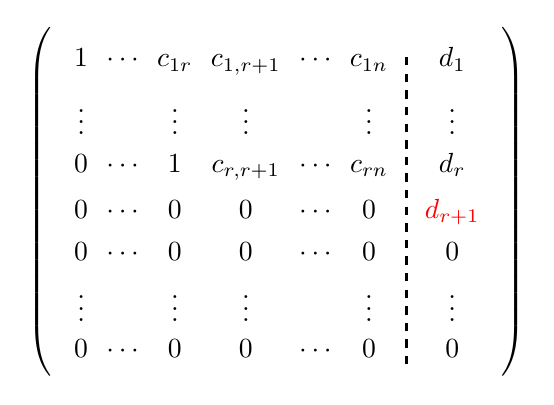
\begin{tikzpicture}
    \matrix(MM) [matrix of math nodes,nodes in empty cells,ampersand replacement=\&,left delimiter=(,right delimiter=)] {
      1\&\cd\&c_{1r}\&c_{1,r+1}\&\cd\&c_{1n}\&\&d_1\\        
      \vd\&\&\vd\&\vd\&\&\vd\&\&\vd\\
      0\&\cd\&1\&c_{r,r+1}\&\cd\&c_{rn}\&\&d_r\\
      0\&\cd\&0\&0\&\cd\&0\&\&\red{d_{r+1}}\\
      0\&\cd\&0\&0\&\cd\&0\&\&0\\        
      \vd\&\&\vd\&\vd\&\&\vd\&\&\vd\\
      0\&\cd\&0\&0\&\cd\&0\&\&0\\
    };  
    \draw[thick,dashed] (MM-1-7.north)--(MM-7-7.south);
  \end{tikzpicture}
\end{center}
其中$d_{r+1}\ne 0$(否则$\rank(\MA,\vb)=r$)。这意味着出现了矛盾方程
$$
0 = \red{d_{r+1}}.
$$    
\end{frame}

\begin{frame}
\begin{tuilun}
  $$
  \MA\vx=\vb\mbox{有唯一解} ~~\Longleftrightarrow~~
  \rank(\MA,\vb)=\rank(\MA)=\MA\mbox{的列数}.
  $$
\end{tuilun}
\begin{center}
  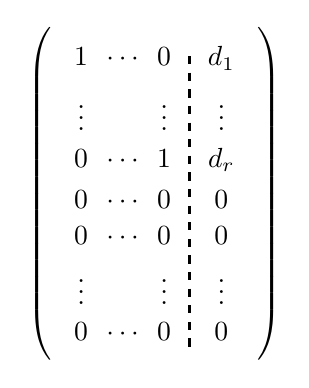
\begin{tikzpicture}
    \matrix(MM) [matrix of math nodes,nodes in empty cells,ampersand replacement=\&,left delimiter=(,right delimiter=)] {
      1\&\cd\&0\&\&d_1\\        
      \vd\&\&\vd\&\&\vd\\
      0\&\cd\&1\&\&d_r\\
      0\&\cd\&0\&\&0\\
      0\&\cd\&0\&\&0\\
      \vd\&\&\vd\&\&\vd\\
      0\&\cd\&0\&\&0\\
    };  
    \draw[thick,dashed] (MM-1-4.north)--(MM-7-4.south);
  \end{tikzpicture}
\end{center}
\end{frame}

\begin{frame}
\begin{dingli}
  若$\vx_1,~\vx_2$是$\MA\vx=\vb$的解,则$\vx_1-\vx_2$是$\MA\vx=\M0$的解。
\end{dingli}
\pause 
\begin{proof}
$$
\MA(\vx_1-\vx_2)=\MA\vx_1-\MA\vx_2=\vb-\vb=\M0,
$$
故$\vx_1-\vx_2$是$\MA\vx=\M0$的解。
\end{proof}
\end{frame}

\begin{frame}
\begin{dingli}
  若$\MA\vx=\vb$有解,则其一般解(或称通解)为
  $$
  \vx=\vx_0+\bar\vx
  $$
  其中$\vx_0$是$\MA\vx=\vb$的一个特解,而
  $$
  \bar\vx=k_1\vx_1+k_2\vx_2+\cd+k_p\vx_p
  $$
  为$\MA\vx=\M0$的一般解。
\end{dingli}
\pause 
\begin{proof}
  $$
  \MA(\vx_0+\bar\vx)=\MA\vx_0+\MA\bar\vx=\vb ~~\Rightarrow~~
  \vx_0+\bar\vx\mbox{是}\MA\vx=\vb\mbox{的解}
  $$
  设$\vx^*$是$\MA\vx=\vb$的任意一个解,则$\vx^*-\vx_0$是$\MA\vx=\M0$的解,而
  $$
  \vx^*=\vx_0+(\vx^*-\vx_0).
  $$
  故$\vx^*$可表示为$\vx_0+\bar\vx$的形式。
\end{proof}
\end{frame}

\begin{frame}
非齐次线性方程组
$$\MA\vx=\vb$$
的通解为
$$
k_1\vx_1+k_2\vx_2+\cd+k_p\vx_p + \red{\vx_0}
$$
其中$\vx_1,\vx_2,\cd,\vx_p$为$\MA\vx=\M0$的基础解系,$\vx_0$为$\MA\vx=\vb$的一个特解。
\end{frame}

\begin{frame}
\begin{zhu}
  “$\MA\vx=\vb$的通解” =  “$\MA\vx=\M0$的通解” + “$\MA\vx=\vb$的特解”
\end{zhu}
\end{frame}

\begin{frame}
\begin{li}
  求非齐次线性方程组$\MA\vx=\vb$的一般解,其中增广矩阵为
  $$
  (\MA,\vb) = \left(
    \begin{array}{rrrrr}
      1&-1&-1& 1&\red{0}\\
      1&-1& 1&-3&\red{1}\\
      1&-1&-2& 3&\red{-\frac12}
    \end{array}
  \right)
  $$
\end{li}
\end{frame}

\begin{frame}[allowframebreaks]
\begin{jie}
  $$
  \begin{array}{rl}
    \left(
    \begin{array}{rrrrr}
      1&-1&-1& 1&\red{0}\\
      1&-1& 1&-3&\red{1}\\
      1&-1&-2& 3&\red{-\frac12}
    \end{array}
                  \right)  \xlongrightarrow[r_3-r_1]{r_2-r_1} &
                                                                \left(
                                                                \begin{array}{rrrrr}
                                                                  1&-1&-1& 1&\red{0}\\
                                                                  0& 0& 2&-4&\red{1}\\
                                                                  0& 0&-1& 2&\red{-\frac12}
                                                                \end{array}
                                                                              \right) \\[0.4in]
    \xlongrightarrow[r_2\div2]{r_1-r_3,r_3+\frac12r_2} &
                                                         \left(
                                                         \begin{array}{rrrrr}
                                                           1&-1&-1& 1&\red{0}\\
                                                           0& 0& 1&-2&\red{\frac12}\\
                                                           0& 0& 0& 0&\red{0}
                                                         \end{array}
                                                                       \right)
  \end{array}
  $$
  同解方程为
  $$
  \left\{
    \begin{array}{rcrcrcr}
      x_1&=&x_2&+&x_4&+&\frac12\\[0.1in]
      x_3&=&&&2x_4&+&\frac12
    \end{array}
  \right.
  $$
  亦即
  $$
  \left\{
    \begin{array}{rcrcrcr}
      x_1&=&x_2&+&x_4&+&\frac12\\[0.1in]
      x_2&=&x_2&&&&\\[0.1in]
      x_3&=&&&2x_4&+&\frac12\\[0.1in]
      x_4&=&&&x_4&&
    \end{array}
  \right.
  $$
  故通解为
  $$
  \left(
    \begin{array}{c}
      x_1\\x_2\\x_3\\x_4
    \end{array}
  \right) = c_1    \left(
    \begin{array}{c}
      1\\1\\0\\0
    \end{array}
  \right)+c_2    \left(
    \begin{array}{c}
      1\\0\\2\\1
    \end{array}
  \right)+    \left(
    \begin{array}{c}
      1/2\\0\\1/2\\0
    \end{array}
  \right) \quad c_1,c_2\in\mathbb R
  $$
\end{jie}
\end{frame}

\begin{frame}
\begin{li}[重要题型]
  设有线性方程组
  $$
  \left\{
    \begin{array}{rrrcr}
      (1+\lambda)x_1&+x_2&+x_3&=&0\\[0.05in]
      x_1&+(1+\lambda)x_2&+x_3&=&3\\[0.05in]
      x_1&+x_2&+(1+\lambda)x_3&=&\lambda
    \end{array}
  \right.
  $$
  问$\lambda$取何值时,此方程组
  \begin{itemize}
  \item[(1)]有唯一解?
  \item[(2)]无解? 
  \item[(3)]有无穷多解? 并在有无穷多解时求其通解。
  \end{itemize}
\end{li}
\end{frame}

\begin{frame}[allowframebreaks]
\begin{jie}
  $$
  |\MA|=\left|
    \begin{array}{ccc}
      1+\lambda&1&1\\
      1&1+\lambda&1\\
      1&1&1+\lambda
    \end{array}
  \right| = (3+\lambda)\lambda^2.
  $$
  故当$\lambda\ne0$且$\lambda\ne-3$时,有唯一解。
  当$\lambda=0$时,原方程组为
  $$
  \left\{
    \begin{array}{l}
      x_1+x_2+x_3=0,\\
      x_1+x_2+x_3=3,\\
      x_1+x_2+x_3=0      
    \end{array}
  \right.
  $$
  它为矛盾方程组,故无解。 \vspace{0.1in}

  当$\lambda=-3$时,增广矩阵为
  $$
  \left(
    \begin{array}{rrrr}
      -2&1&1&\red{0}\\
      1&-2&1&\red{3}\\
      1&1&-2&\red{-3}
    \end{array}
  \right) \xlongrightarrow[]{\mbox{初等行变换}}
  \left(
    \begin{array}{rrrr}
      1&0&-1&\red{-1}\\
      0&1&-1&\red{-2}\\
      0&0&0&\red{0}
    \end{array}
  \right)
  $$
  得同解方程组为
  $$
  \left\{
    \begin{array}{l}
      x_1=x_3-1\\[0.05in]
      x_2=x_3-2\\[0.05in]
      x_3=x_3
    \end{array}
  \right.
  $$
  通解为
  $$
  \left(
    \begin{array}{c}
      x_1\\x_2\\x_3
    \end{array}
  \right) = c\left(
    \begin{array}{c}
      1\\1\\1
    \end{array}
  \right)+\left(
    \begin{array}{r}
      -1\\-2\\0
    \end{array}
  \right) \quad c\in\mathbb R
  $$
\end{jie}
\end{frame}

\begin{frame}
\begin{li}
  设$\etabd^*$为$\MA\vx=\vb$的一个解,$\xibd_1,~\xibd_2,~\cd,~\xibd_{n-r}$为对应的齐次线性方程组的一个基础解系,证明:
  \begin{itemize}
  \item[(1)] $\etabd^*,~\xibd_1,~\xibd_2,~\cd,~\xibd_{n-r}$线性无关;
  \item[(2)] $\etabd^*,~\etabd^*+\xibd_1,~\etabd^*+\xibd_2,~\cd,~\etabd^*+\xibd_{n-r}$线性无关。
  \end{itemize}
\end{li}
\end{frame}

\begin{frame}
\begin{proof}
\begin{itemize}
\item[(1)] 假设$\etabd^*,~\xibd_1,~\xibd_2,~\cd,~\xibd_{n-r}$线性相关,而$\xibd_1,~\xibd_2,~\cd,~\xibd_{n-r}$线性无关,故$\etabd^*$可由$\xibd_1,~\xibd_2,~\cd,~\xibd_{n-r}$线性表示,从而$\etabd^*$为$\MA\vx=\M0$的解,这与$\etabd^*$为$\MA\vx=\vb$的解矛盾。故假设不成立,即$\etabd^*,~\xibd_1,~\xibd_2,~\cd,~\xibd_{n-r}$线性无关。 
\item[(2)] 显然,
  $$\etabd^*,~\xibd_1,~\xibd_2,~\cd,~\xibd_{n-r}
  \mbox{~~等价于~~} 
  \etabd^*,~\etabd^*+\xibd_1,~\etabd^*+\xibd_2,~\cd,~\etabd^*+\xibd_{n-r},$$  
  由题(1)结论可知
  $$
  \begin{aligned}
    &\rank(\etabd^*,~\etabd^*+\xibd_1,~\etabd^*+\xibd_2,~\cd,~\etabd^*+\xibd_{n-r})\\
    =& 
    \rank(\etabd^*,~\xibd_1,~\xibd_2,~\cd,~\xibd_{n-r}) = n-r+1
  \end{aligned}
  $$
  从而结论成立。
\end{itemize}
\end{proof}
\end{frame}

\begin{frame}
\begin{li}
  设$\etabd_1,~\etabd_2,~\cd,~\etabd_s$为$\MA\vx=\vb$的$s$个解,$k_1,~k_2,~\cd,~k_{s}$为实数,满足$k_1+k_2+\cd+k_s=1$。证明:
  $$
  \vx=k_1\etabd_1+k_2\etabd_2+\cd+k_s\etabd_s
  $$
  也是它的解。
\end{li} \pause 
\begin{proof}
$$
\begin{array}{rcl}
  \MA(k_1\etabd_1+k_2\etabd_2+\cd+k_{s}\etabd_{s})&=&
                                                     k_1\MA\etabd_1+k_2\MA\etabd_2+\cd+k_s\MA\etabd_s\\[0.05in]
                                                 &=&k_1\vb+k_2\vb+\cd+k_s\vb\\[0.05in]
                                                 &=&\vb.
\end{array}
$$
\end{proof}
\end{frame}

\begin{frame}
\begin{li}
  对于$\MA\vx=\vb$,$\rank(\MA)=r$,$\etabd_1,~\etabd_2,~\cd,~\etabd_{n-r+1}$为它的$n-r+1$个线性无关的解。证明它的任一解可表示为
  $$
  \vx=k_1\etabd_1+k_2\etabd_2+\cd+k_{n-r+1}\etabd_{n-r+1},
  $$
  其中$k_1+k_2+\cd+k_{n-r+1}=1$
\end{li}
\end{frame}

\begin{frame}[allowframebreaks]
\begin{proof}
取向量组
$
\blue{\etabd_2-\etabd_1,~~\etabd_2-\etabd_1,~~\cd,~\etabd_{n-r+1}-\etabd_1.}
$
下证该向量组为$\MA\vx=\M0$的一个基础解系。 
$$
(\etabd_1,~\etabd_2,~\cd,~\etabd_{n-r+1}) \xlongrightarrow[j=2,\cd,n-r+1]{c_j-c_1}
(\etabd_1,~\etabd_2-\etabd_1,~\cd,~\etabd_{n-r+1}-\etabd_1)
$$ 
$$
\begin{array}{rl}
  &\etabd_1,~\etabd_2,~\cd,~\etabd_{n-r+1}\mbox{线性无关}\\[0.1in]  
  \Rightarrow&\etabd_1,~\etabd_2-\etabd_1,~\cd,~\etabd_{n-r+1}-\etabd_1\mbox{线性无关}\\[0.1in]  
  \Rightarrow&\etabd_2-\etabd_1,~\cd,~\etabd_{n-r+1}-\etabd_1\mbox{线性无关}\\[0.1in]  
  \Rightarrow& \etabd_2-\etabd_1,~\cd,~\etabd_{n-r+1}-\etabd_1\mbox{为}\MA\vx=\M0
               \mbox{的基础解系}.      
\end{array}
$$
于是$\MA\vx=\vb$的任意一个解$\vx$可表示为
$$
\begin{array}{rl}
  & \vx = k_2(\etabd_2-\etabd_1)+\cd+k_{n-r+1}(\etabd_{n-r+1}-\etabd_1)+\red{\etabd_1}\\[0.1in] 
  \Rightarrow & 
                \vx = (1-k_2-\cd-k_{n+r-1})\etabd_1+k_2\etabd_2+\cd+k_{n-r+1}\etabd_{n-r+1}\\[0.1in]
  \Rightarrow & 
                \vx =k_1\etabd_1+k_2\etabd_2+\cd+k_{n-r+1}\etabd_{n-r+1}
\end{array}
$$
\end{proof}
\end{frame}


\begin{frame}
\begin{li}
  设四元齐次线性方程组
  $$
  (I):\left\{
    \begin{array}{l}
      x_1+x_2=0,\\
      x_2-x_4=0;
    \end{array}
  \right. \quad
  (II):\left\{
    \begin{array}{l}
      x_1-x_2+x_3=0,\\
      x_2-x_3+x_4=0.
    \end{array}
  \right.
  $$
  求
  \begin{itemize}
  \item[(1)] 方程组$(I)$与$(II)$的基础解系
  \item[(2)] 方程组$(I)$与$(II)$的公共解        
  \end{itemize}
\end{li}
\end{frame}

\begin{frame}
\begin{jie}
  (1)、因为
    $$
    (I) \Longleftrightarrow
    \left\{
      \begin{array}{rcr}
        x_1&=&-x_2\\[0.05in]
        x_4&=&x_2
      \end{array}
    \right. \Longleftrightarrow
    \left\{
      \begin{array}{rcrr}
        x_1&=&-x_2&\\[0.05in]
        x_2&=&x_2&\\[0.05in]
        x_3&=&&x_3\\[0.05in]
        x_4&=&x_2&
      \end{array}
    \right. 
    $$   
    故$(I)$的基础解系为
    $$
    \xibd_1=\left(
      \begin{array}{r}
        -1\\1\\0\\1
      \end{array}
    \right), \quad
    \xibd_2=\left(
      \begin{array}{r}
        0\\0\\1\\0
      \end{array}
    \right)
    $$
  \end{jie}
  \end{frame}

\begin{frame}
\begin{jie}[续]
  因为
  $$
  (II) \Longleftrightarrow
  \left\{
    \begin{array}{rcrr}
      x_1&=&x_2&-x_3\\[0.05in]
      x_4&=&-x_2&+x_3
    \end{array}
  \right. \Longleftrightarrow
  \left\{
    \begin{array}{rcrr}
      x_1&=&x_2&-x_3\\[0.05in]
      x_2&=&x_2&\\[0.05in]
      x_3&=&&x_3\\[0.05in]
      x_4&=&-x_2&+x_3
    \end{array}
  \right. 
  $$
  故$(II)$的基础解系为
  $$
  \xibd_1=\left(
    \begin{array}{r}
      1\\1\\0\\-1
    \end{array}
  \right), \quad
  \xibd_2=\left(
    \begin{array}{r}
      -1\\0\\1\\1
    \end{array}
  \right)
  $$
\end{jie}
\end{frame}

\begin{frame}
\begin{jie}[续]
  (2)、 方程$(I)$与$(II)$的公共解即为联立$(I)$与$(II)$所得新方程组的解:
    $$
    \left\{
      \begin{array}{l}
        x_1+x_2=0\\
        x_2-x_4=0\\
        x_1-x_2+x_3=0\\
        x_2-x_3+x_4=0
      \end{array}
    \right.
    $$
\end{jie}
\end{frame}

\begin{frame}
\begin{jie}[续]

    $$
    \begin{array}{rl}
      \left(
      \begin{array}{rrrr}
        1&1&0&0\\
        0&1&0&-1\\
        1&-1&1&0\\
        0&1&-1&1
      \end{array}
                \right) \xlongrightarrow[r_3-r_1]{r_4+r_2} & 
                                                             \left(
                                                             \begin{array}{rrrr}
                                                               1&1&0&0\\
                                                               0&1&0&-1\\
                                                               0&-2&1&0\\
                                                               0&2&-1&0
                                                             \end{array}
                                                                       \right) \\[0.3in]
      \xlongrightarrow[r_3\times(-1)]{r_3+r_4}&
                                                \left(
                                                \begin{array}{rrrr}
                                                  1&1&0&0\\
                                                  0&1&0&-1\\
                                                  0&2&-1&0\\
                                                  0&0&0&0
                                                \end{array}
                                                         \right)         
    \end{array}
    $$  
    即
    $$
    \left\{
      \begin{array}{rcr}
        x_1&=&-x_2\\
        x_2&=&x_2\\
        x_3&=&2x_2\\
        x_4&=&x_2
      \end{array}
    \right.  ~~ \Rightarrow ~~
    \vx = c\left(
      \begin{array}{r}
        -1\\1\\2\\1
      \end{array}
    \right) \quad c\in \mathbb R.
    $$
\end{jie}
\end{frame}






\end{document}
